\chapter{Baryonic Structures}


\section{State and distribution of baryons}


We want to include baryons in the study of non-linear structure formation.

\subsection{Evolution}
Before recombination and decoupling, the baryons were an ionized plasma.

After recombination, they are mostly neutral and in atomic form. At that point, there is little emission, which is why this period is called the Dark Ages.

At later times ($z \approx 6$ -- $20$), the first astrophysical objects start to form (like stars, galaxies, etc.), which emit UV photons that re-ionize the baryons and end the Dark Ages. This is called the Epoch of Reionization (EoR).

Following this, the baryons continue to participate in structure formation, driven by dark matter.



\subsection{Phases}

\begin{itemize}[nolistsep]
	\item Gas
	\begin{itemize}
		\item Hot gas (ionized)
		\item Cold gas (atomic or molecular form)
	\end{itemize}
	\item Stars
\end{itemize}
These different phases interact and convert to each other.



\subsection{Distribution}
\newacronym{ism}{ISM}{interstellar medium}
\newacronym{igm}{IGM}{intergalactic medium}
\newacronym{icm}{ICM}{intra-cluster medium}
\begin{itemize}
	\item within galaxies: \Ac{ism}
	\item between galaxies: \Ac{igm}
	\item within galaxies clusters: \Ac{icm}
\end{itemize}




\subsection{Dynamics}
We know that there is five times as much dark matter mass as there is baryonic mass.
As a result, dark matter mostly drives the dynamics of structure formation and provides the backbone for the dynamics of the baryons.
Unlike dark matter, baryons are collisional, and their dynamics include various effects:
\begin{itemize}
	\item Thermodynamical effects: Heating and cooling
	\item Radiative transfer: Interaction between baryons and photons
	\item Hydrodynamical effects: Shocks
	\item Transitions between different phases: Star formation
	\item Astrophysical effects: Supernova explosions and active galactic nuclei
\end{itemize}
The dynamics of baryons is more complicated than that of dark matter.
Figure \ref{fig:illustris-evolution} shows the evolution of dark matter and ordinary matter from a simulation.

\begin{figure}
	\includegraphics[width=\textwidth]{img/ch-05/illustris-evolution.png}
	\caption{The evolution of dark matter and ordinary matter from the illustris simulation.}
	\label{fig:illustris-evolution}
\end{figure}

Generally, some baryons tend to sink to the bottom of potential wells driven by dark matter on small scales, because baryons have dissipation.

Our approach here is to first review astrophyiscal facts about baryonic structures and discuss approaches for modelling the baryons.





\section{Stars}

Stars are formed by the collapse of cold gas in molecular clouds in the ISM.
They are supported against gravity by nuclear fusion reactions at their centre.
The energy that is produced is transported outwards by photons to the star's outer shells.

\subsection{Sun}
We have already seen that $M_\sol \approx \SI{2e30}{\kg}$.


\subsection{Composition}
\begin{table}
	\begin{tabular}{lccccccccc}
	\toprule
	Element & H & He & C & N & O & Ne & Mg & Si & Fe\\
	\midrule
	$(N/N_H) \cdot 10^5$ & $10^5$ & 9800 & 36.3 & 11.2 & 85.1 & 12.3 & 3.80 & 3.55 & 4.68\\
	\bottomrule
	\end{tabular}
	\caption{The chemical composition of the sun.}
	\label{tab:solar-comp}
\end{table}
The solar composition is shown in \cref{tab:solar-comp}.
For comparison, the primordial abundance is about \SI{75}{\percent} hydrogen and \SI{25}{\percent} helium, with only traces of heavier elements.
Apparently, the abundance of helium and heavier elements in the sun is different from the primordial abundance.
This is because heavier elements are produced by nuclear reactions in stars.
To characterize these abundances, we define the \emph{metallicity} $Z$, which is the mass faction of elements heavier than helium.
For the sun, $Z_\sol \approx \SI{2}{\percent}$.

Stellar types are classified based on their surface temperature, which is shown in TODO.
The spectra of different types are shown in TODO.


\subsection{Classification}
\begin{margintable}
	\begin{tabular}{ll}
		\toprule
		Class & $T$ [K]\\
		\midrule
		O & \num{28000}--\num{50000}\\
		B & \num{10000}--\num{28000}\\
		A & \num{7500}--\num{10000}\\
		F & \num{6000}--\num{7500}\\
		G & \num{5000}--\num{6000}\\
		K & \num{3500}--\num{5000}\\
		M & \num{2500}--\num{3500}\\
		\bottomrule
	\end{tabular}
	\caption{The spectral type as a function of temperature.}
	\label{tab:spectral-type}
\end{margintable}
The modern classification system for stars is the MK classification, which consists of a spectral classification and a luminosity classification.

The spectral classification is a single letter for rough classification, followed optionally by a single number for finer classification.
\Cref{tab:spectral-type} shows the temperature of stars with different spectral types. The mass of a star depends on its temperature. The hotter a star is, the more massive it is. 

\subsection{Hertzsprung-Russel diagram}

\newacronym{hr}{HR}{Hertzsprung-Russel}
The \ac{hr} diagram in \cref{fig:hr-gaia} shows the relationship between surface temperature and luminosity of stars in our galaxy.

\begin{figure}
	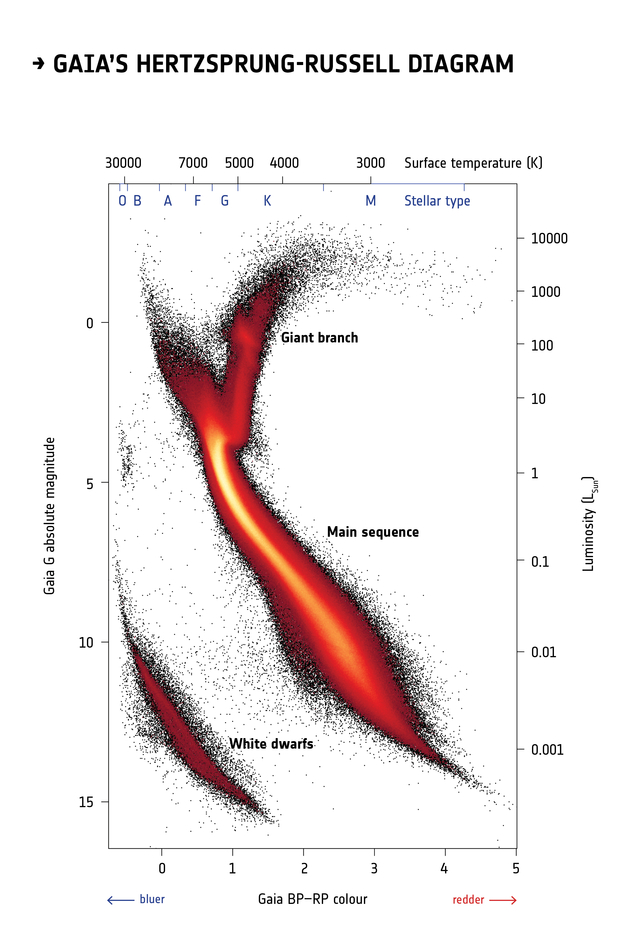
\includegraphics[width=\textwidth]{img/ch-05/hr-gaia.png}
	\caption{The Hertzsprung-Russell diagram, as measured by the GAIA satellite.}
	\label{fig:hr-gaia}
\end{figure}

\newacronym{ms}{MS}{main sequence}
\newacronym{imf}{IMF}{initial mass function}
\newacronym{rgb}{RGB}{red giant branch}
The evolution of stars can be tracked on the \ac{hr} diagram.
Stars are born on the \ac{ms}.
The phenomenological \ac{imf} is the distribution of newly born stars of the \ac{ms}.
Eventually, they have burned all their hydrogen and start moving away from the \ac{ms} towards the \ac{rgb}.
Stars with higher masses exhaust their hydrogen first.
As a reg giant runs out of nuclear fuel, they collapse into compact objects. Depending on their mass, this compact object can be a white dwarf, a neutron star, or a black hole.
In the process, supernova explosions can be generated.
They inject kinetic energy into the \ac{ism} and disperse the heavy elements that the star generated.
This process is called enrichment of the \ac{ism}.


\subsection{Galaxies}
Galaxies contain many stars, so they can be used to track the stellar evolution.
Because the massive blue stars burn their fuel first, new galaxies are blue, and old galaxies are red.



\section{Classification of galaxies}

\begin{figure}
	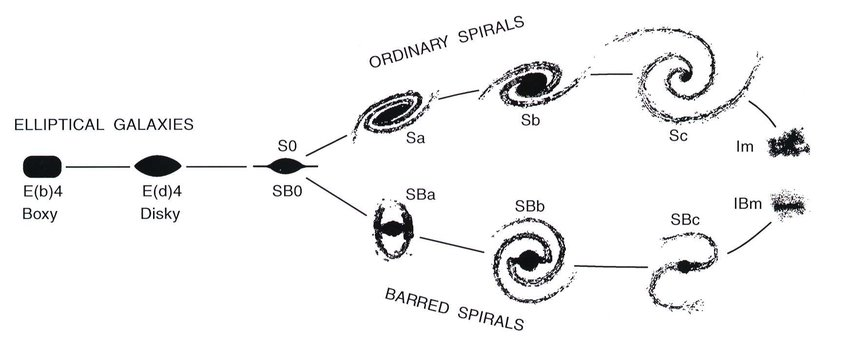
\includegraphics[width=\textwidth]{img/ch-05/tuning-fork.jpg}
	\caption{The Hubble tuning fork diagram classifies galaxies according to their shape.}
	\label{fig:tuning-fork}
\end{figure}

There is a wide range of types of galaxies.
A common classification is the Hubble sequence, also known as the tuning fork diagram, which is shown in \cref{fig:tuning-fork}.
The Hubble sequence distinguishes the following types:
\begin{itemize}
	\item Elliptical galaxies have a smooth elliptical light distribution. They are subdivided into E0 (spherical) to E7 (very flat).
	\item Spiral galaxies have a disk with spiral arms, and a central halo.
	\begin{itemize}
		\item Normal spiral galaxies go from Sa (tight spiral and relatively faint HII regions) to Sc (loose spiral and bright HII regions).
		\item Barred spiral galaxies go from SBa (tight spiral and relatively faint HII regions) to SBc (loose spiral and bright HII regions).
	\end{itemize}
	\item Lenticular galaxies (S0) are an intermediate step between ellipticals and spirals. They have a smooth light distribution with no spiral arms and a thin disk with a bulge. 
\end{itemize}
There are also other types of galaxies which are not on the Hubble sequence:
\begin{itemize}
	\item Irregular galaxies have irregular shapes.
	\item Peculiar galaxies have odd shapes and are often associated with mergers.
	\item Dwarf galaxies are galaxies with luminosities fainter than $M_B = -18$.
	\item Active galactic nuclei are very bright nuclei that can be found in some galaxies. They may be the only part of an otherwise faint galaxy that is visible to us.
\end{itemize}

Elliptical galaxies are called \enquote{early types}, and spirals are called \enquote{late types}.
The nomenclature is historical and is not related to the formation history.



% 5.4
\section{Elliptical galaxies}
Elliptical galaxies tend to be regular, with a smooth elliptical light distribution.

\subsection{Surface brightness}
The surface brightness of elliptical galaxies is well fit by a \emph{Sérsic profile},
\begin{align*}
	I(R)
	&= I_0 \exp\Bigg[ - \beta_n \left( \frac{R}{R_e}  \right)^{1/n} \Bigg],
\end{align*}
where $m$ is the Sérsic index,
$R$ is the semi-major axis length,
$R_e$ is the half-light radius,
and it follows that $\beta_n \approx 2 n - 0.324$ to fulfill this criterion.
The brighter galaxies have a larger value of $n$.
For normal ellipticals, $n \approx 4$, for which the profile is also called a \emph{de Vaucouleurs profile}.

\subsection{Shape}
Let $b/a$ be the ratio of minor to major axis of the light distribution.
For normal ellipticals, $b/a \in [0.3, 1]$.
In the Hubble sequence, this corresponds to types E0 to E7.

\subsection{Colour}
Ellipticals tend to be redder than spirals, which indicates an older, metal-rich star population.
Some ellipticals have colour gradients, such that the central regions tend to be redder.

\subsection{Kinematics}
The support against gravitational collapse is mostly provided by random motion.
The rotational velocities are comparatively small.


\subsection{Scaling relations}
\begin{marginfigure}
	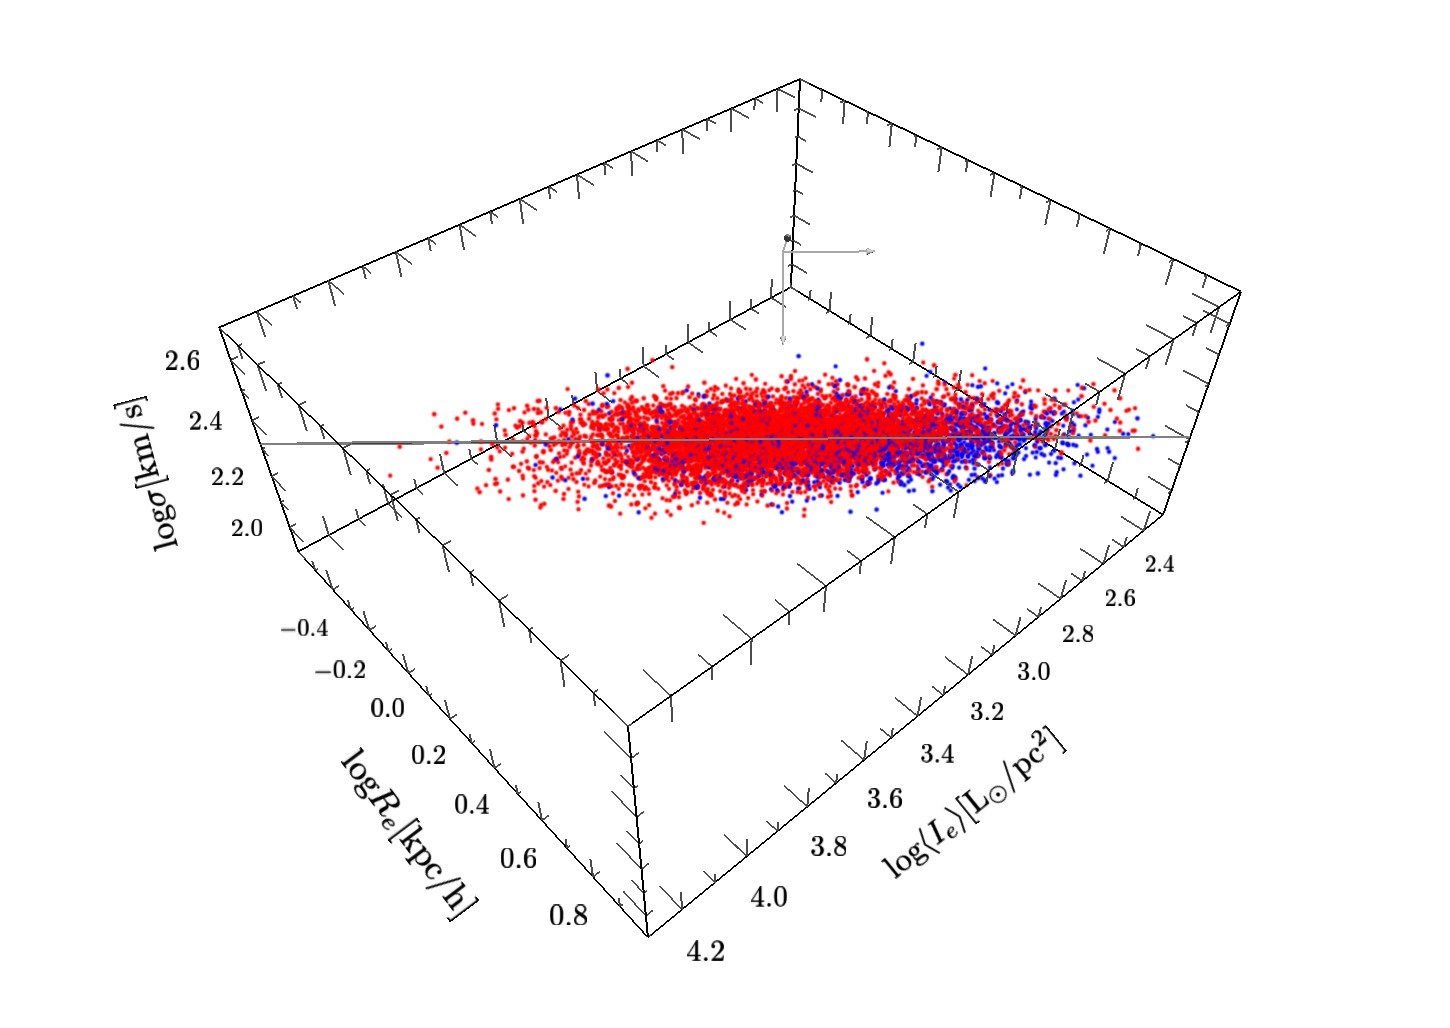
\includegraphics[width=\textwidth]{img/ch-05/fundamental-plane.png}
	\caption{The fundamental plane for elliptical galaxies, from \cite{Magoulas:2012jy}. The view is chosen such that the plane is seen edge-on as a line.}
	\label{fig:fundamental-plane}
\end{marginfigure}
There is a correlation between some of the main characteristics of ellipticals.
Let $\sigma$ be the line of sight velocity dispersion of stars inside the half-light radius $R_e$,
and let $\avg{I}_l$ be the main surface brightness within $R_e$.
\Cref{fig:fundamental-plane} shows the \emph{fundamental plane}, which which quantifies the correlation between these parameters.
The correlation between $\avg{I_l}$ and $\sigma$ is called \emph{Faber-Jackson relation}.
The correlation between $R_e$ and $\sigma$ is called the \emph{$D_n$-$\sigma$ relation}, whose name comes from an other measure for radius, $D_n$.


\subsection{Gas content}
Very little cold gas, with temperatures less than \SI{100}{\kelvin}, is contained in ellipticals.
As a result, new stars are not forming, which explains the old stellar population.
Hot gas with temperatures around \SI{e7}{\kelvin} is much more abundant, and can be found with x-ray observations.
There is also a little warm gas, with temperature \SI{e4}{\kelvin}.







\section{Spiral galaxies}
\begin{marginfigure}
	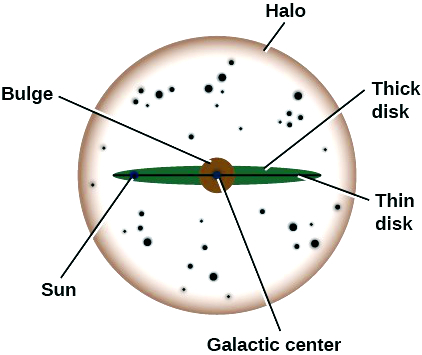
\includegraphics[width=\textwidth]{img/ch-05/milky-way.png}
	\caption{Structure of the Milky Way.}
	\label{fig:mw-structure}
\end{marginfigure}
Spiral galaxies, like the Milky Way in \cref{fig:mw-structure}, show a spiral structure when viewed face-on, and look like a flat disk with a central bulge edge-on.
They also have a dark matter halo, which surrounds and includes the visible structure.

\subsection{Surface brightness}
The disks of spiral galaxies are well fitted by an exponential profile,
\begin{align*}
	I(R)
	&= I_0 \exp\left( -\frac{R}{R_d} \right),
\end{align*}
which is a Sérsic profile with Sérsic index $n=1$,
and $R_e \approx 1.67 R_d$.
More luminous spirals usually have larger radii.
Bulges are also well fitted by a Sérsic profile, with $n = 4$ for large bulges, down to $n=1$ for smaller ones.

\subsection{Colour}
Spirals tend to be blue, which indicates a younger and still forming stellar population in the disk.
More luminous disks tend to be redder.
The star formation rate $\dot{M}_* = \dv*{M_*}{t}$, where $M_*$ is the total mass of stars in a galaxy, varies considerably between galaxies.
Galaxies with very high star formation rates are called \emph{Starburst galaxies}.

The stellar haloes are mostly made up of old metal-poor stars.
More than half of all spiral galaxies have a bar.
The spiral arms are typically bluer and contain regions of star formation.

\subsection{Gas content}
Spirals have mostly cold gas in the disk, which gives them a reservoir for star formation.

\subsection{Kinematics}
\begin{marginfigure}
	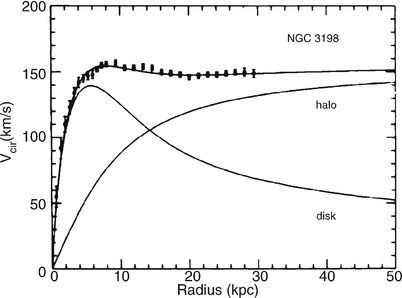
\includegraphics[width=\textwidth]{img/ch-05/rotation-curve.png}
	\caption{The rotation curve of the galaxy NGC 3198. The rotation curve is the result of a contribution from baryonic matter in the disk and a dark matter halo, which extends beyond the disk. The baryonic matter is on average closer to the centre of the galaxy, because unlike dark matter, it can lose energy by dissipation.}
	\label{fig:rotation-curve}
\end{marginfigure}
The disks in spirals are rotationally supported, with approximately circular orbits for stars and gas.
According to Newtonian gravity, the rotational velocity $v_\text{rot}$ of a star at radius $r$ can be found as follows:
\begin{alignat*}{3}
	         && F &= ma\\
	&\implies & \frac{G m M(r)}{r^2} &= m \frac{v_\text{rot}^2}{r}\\
	&\implies & v_\text{rot} &= \sqrt{\frac{G M(r)}{r}}.
\end{alignat*}
\Cref{fig:rotation-curve} is the rotation curve of the galaxy NGC 3198, which shows that the rotational velocity as a function of radius rises quickly and then remains flat, which cannot be explained from the visible matter alone, since we would expect a fall-off of the rotational velocity along with the brightness profile.
Apparently, there must be another invisible contribution to the mass, which comes from the dark matter halo.
For $v_\text{rot}$ to be constant, we need $M(r) \propto r$, which implies $\rho(r) \propto r^{-2}$.
The NFW profile at intermediate radii is a good model for this.

\subsection{Scaling relations}
The correlation between the maximal rotational velocity $v_\text{max}$ and the luminosity $L$ is well fitted by
\begin{align*}
	L = A v_\text{max}^\alpha, 
	\qquad \text{with } \alpha \in [2.5, 4],
\end{align*}
which is called the \emph{Tully-Fisher relation}.




\section{Dwarf galaxies}
Dwarf galaxies are galaxies with low luminosities, such that $M_B \geq - 18$.
\Cref{fig:dwarfs} shows that they can have diverse structures, and they can be separated into different subtypes.
\begin{itemize}
	\item Dwarf galaxies that are gas rich, show strong star formation, and have irregular shapes are called \emph{Dwarf irregulars}, dIrr.
	\item Dwarf galaxies that are gas poor, without young stars, and with regular structures, are subdivided into \emph{Dwarf ellipticals}, dE, and the fainter Dwarf spheroidals, dSph.
\end{itemize}


\section{Active galactic nuclei}
\newacronym[longplural={active galactic nuclei}]{agn}{AGN}{active galactic nucleus}
\Acp{agn} are very luminous centres that can be found in some galaxies, which are then called \emph{active galaxies}.
Observationally, they come in different subclasses, some of them being Seyfert galaxies, quasars, blazars, radio \ac{agn}, and liners.

The spectra of \acp{agn} are very different from what one would expect from stellar sources, since they emit strongly across the entire range of the electromagnetic spectrum, from the radio to the gamma ray range, and they contain strong emission lines.

The emission is variable on a time scale of a few days, so for the emission region to be causally connected, it must be smaller than a few light days.
This is a very compact length scale compared to the rest of the galaxy.

\newacronym{smbh}{SMBH}{supermassive black hole}
\Acp{agn} are powered by accretion onto a \ac{smbh}, with masses around \SIrange{e6}{e9}{\solarmass}.
The \ac{smbh} grows as it accretes gas, and it can also reinject energy into the \ac{igm} in the form of jets.
Accretion can be a very efficient process to convert gravitational energy into radiation.
While most galaxies, including the Milky Way, have an \ac{smbh} in their centre, they are not necessarily \emph{active} galaxies.

The wide range of types of \acp{agn} can be squeezed reasonably well into unification models, which state that they are all roughly similar kinds of objects, but observed from different viewing angles.

\section{Statistical properties of the galaxy population}

\subsection{Luminosity function}
The luminosity function $\phi(L) \dd{L}$ is defined as the number density of galaxies with luminosities between $L$ and $L + \dd{L}$.
For a wide range of galaxies, a \emph{Schechter function} is a good fit:
\begin{align*}
	\phi(L) \dd{L}
	&= \phi^* \left( \frac{L}{L^*} \right)^\alpha
	\exp\left( - \frac{L}{L^*} \right)
	\frac{\dd{L}}{L^*},
\end{align*}
where
$L^*$ is a characteristic luminosity,
$\alpha$ is the faint end slope,
and $\phi^*$ is a normalization factor.
In \cref{fig:lum-func}, the luminosity function has been fitted to experimental data.
\begin{figure}
	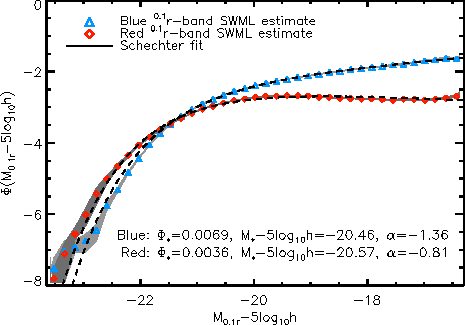
\includegraphics[width=0.7\textwidth]{img/ch-05/luminosity-function.pdf}
	\caption{The r-band SDSS DR6 Luminosity Function for blue and red galaxies separately, from \cite{Montero_Dorta_2009}. The Stepwise Maximum Likelihood Luminosity Function estimates are shown in diamonds. The dashed line represents the best-fit Schechter function. Shaded regions represent the $1 \sigma$ uncertainty.}
	\label{fig:lum-func}
\end{figure}

\subsection{Colour distribution}
\begin{marginfigure}
	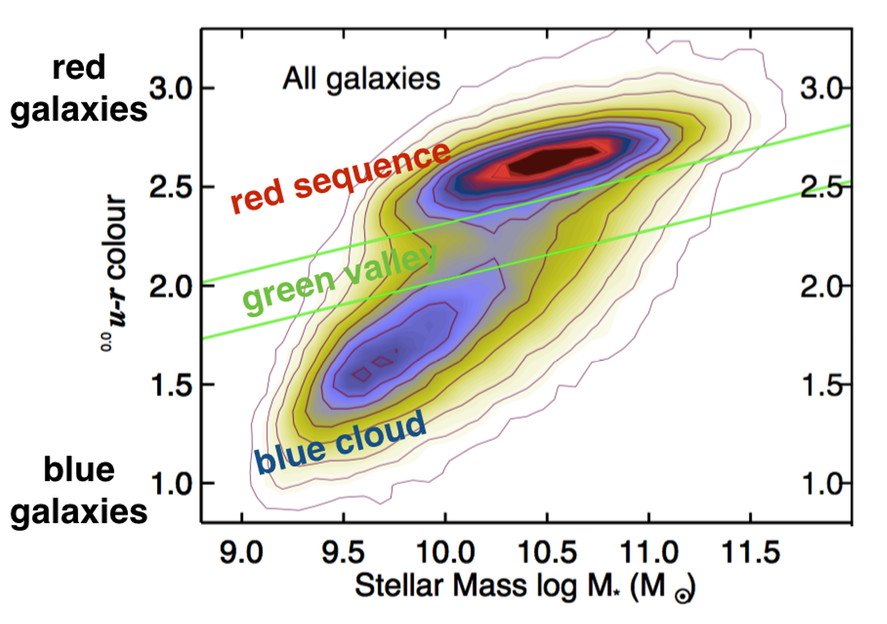
\includegraphics[width=\textwidth]{img/ch-05/cm-galaxies.png}
	\caption{The color-mass diagram for galaxies.}
	\label{fig:cm-galaxies}
\end{marginfigure}
The color-mass diagram for galaxies is shown in \cref{fig:cm-galaxies}.
There are two maxima in the distribution: 
The red sequence consists of bright red galaxies,
and the blue cloud consists of faint blue galaxies.

\subsection{Mass-Metalicity}
Spiral galaxies with large total stellar masses $M_*$ tend to have higher metalicities.

\subsection{Clustering}
Galaxies in denser regions are redder.
Equivalently, elliptical galaxies are more clustered than spiral galaxies.
The fraction of different kinds of galaxies is shown as a function of density in \cref{fig:clustering}
\begin{marginfigure}
	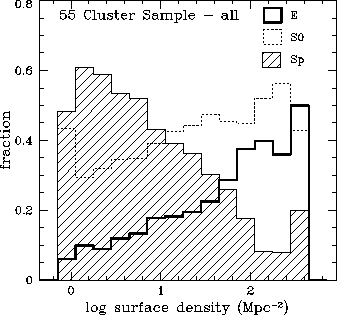
\includegraphics[width=\textwidth]{img/ch-05/clustering.pdf}
	\caption{The fraction of galaxies as a function of morphological density for the D80 55 cluster sample, from \cite{Dressler_1997}.}
	\label{fig:clustering}
\end{marginfigure}







\section{Clusters and groups of galaxies}

\subsection{Clusters of galaxies}
Galaxy clusters are the largest bound objects in the universe.
\begin{itemize}
	\item Number of galaxies: 50 to a few thousand
	\item Radius: a few \si{\mega\parsec}
	\item Mass: \SIrange{e14}{e15}{\solarmass}
	\item Velocity dispersion (line of sight): $\sigma_\text{los} \approx \SI{1000}{\kilo\metre\per\second}$
\end{itemize}

Criteria for selecting clusters:
\begin{itemize}
	\item Richness: The number of galaxy members
	\item Compactness: Number of galaxies within a given radius
	\item Regularity: Circularity or smoothness
\end{itemize}

An example of a survey is the Abell cluster catalogue from 1958.

Nearby clusters are Virgo and Coma.

\paragraph*{Galaxy population}
Clusters are rich in early type (red, elliptical) galaxies.
For regular clusters, \SI{80}{\percent} of galaxies are E or S0, which is higher than the average in the field (outside clusters), about \SI{30}{\percent}.

The fraction of red galaxies tends to decrease in clusters with increasing redshift, which is known as the \emph{Butcher-Oemler effect}.

The radial density of galaxies in clusters is similar to the distribution of dark matter, which indicates that the galaxies act as collisionless particles.

Often, the brightest galaxy in a cluster is very extended, diffuse, and near the centre. They are called cD galaxies, and are thought to have grown through the accretion of multiple galaxies.
The effect is called \emph{galaxy cannibalism}.

\paragraph*{Mass estimation}
There are several techniques to measure the mass of a cluster:
\begin{itemize}
	\item \textbf{Velocity dispersion:}
	Along the line of sight, a velocity dispersion of $\sigma_\text{los} \approx \SI{1000}{\kilo\metre\per\second}$ can be measured with redshift.
	The Virial theorem then yields
	\begin{align*}
		M \approx A \frac{\sigma_\text{los}^2 R}{G},
	\end{align*}
	where the constant $A$ depends on the profile of the cluster and the exact definition of the radius $R$.
	\item \textbf{X-ray emission:}
	The hot gas ($T \approx \SI{e7}{\kelvin}$) in the intra-cluster medium emits bremsstrahlung, which is in the X-ray range.
	If we assume hydrostatic equilibrium, such that the gas is in equilibrium with the gravitational potential, then the X-ray emission profile and the X-ray temperature can be used to derive the total mass of the cluster and the gas.
	\item \textbf{Gravitational lensing:}
	A cluster of galaxies can act as a gravitational lens for the background galaxies.
	The trajectories of photons from distant objects are deflected by the gravitational potential of a cluster.
	The mass of the cluster can be derived from the strength of distortion of the background galaxies.
\end{itemize}

One finds that the mass of clusters is in the range \SIrange{e14}{e15}{\solarmass}.
Also, only \SI{10}{\percent} of the mass is baryonic in nature, which is strong evidence for the existence of dark matter.





\subsection{Groups of galaxies}
\begin{itemize}
	\item Number of galaxies: 3 to 30
	\item Radius: \SIrange{0.1}{1}{\mega\parsec}
	\item Mass: \SIrange{e12.5}{e14}{\solarmass}
	\item Velocity dispersion: $\sigma_\text{los} \approx \SI{300}{\kilo\metre\per\second}$
\end{itemize}

\newacronym{smc}{SMC}{small Magellanic cloud}
\newacronym{lmc}{LMC}{large Magellanic cloud}
An example is the local group, with its largest member, the Milky Way.
There are many Milky Way satellites, such as the \ac{smc} and the \ac{lmc}.
Another large galaxy in the local groups is the Andromeda galaxy (M31).






\section{Intergalactic medium}

The \ac{igm} is made up of the baryons between galaxies.
It is usually too diffuse and not hot enough to be studied in emission,
but it can be seen in absorption.

\subsection{Quasar absorption lines}
Suppose a distant quasar is at redshift $z_q$, and clouds of \ac{igm} are in front of it at different redshifts $z_i$, with $i = 1, 2, 3, \dots$.
The continuum light of the quasar is absorbed by the clouds, particularly by the strong Lyman-alpha transition, with (rest) wavelength $\lambda_\mathrm{α} = \SI{1216}{\angstrom}$.
We thus see absorption lines at wavelengths $\lambda_\mathrm{α} (1 + z_i)$.

\begin{figure}
	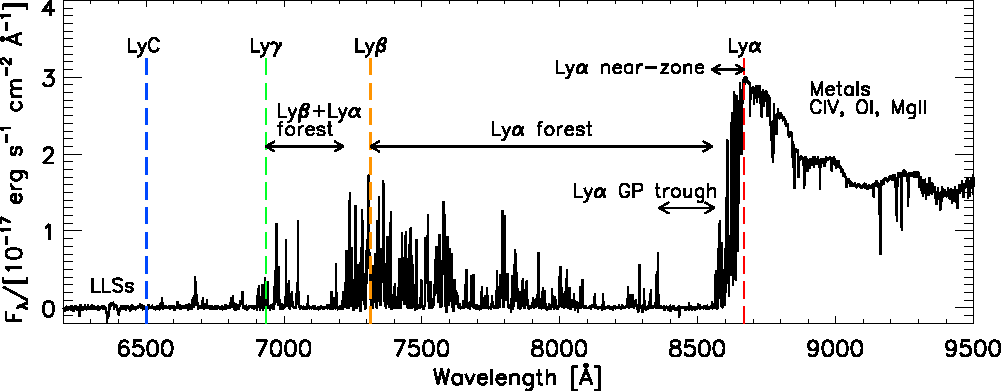
\includegraphics[width=\textwidth]{img/ch-05/quasar-spectrum.pdf}
	\caption{A spectrum of the quasar ULAS J1319+0950 at $z=6.13$ from \cite{becker2015reionization}, obtained with the X-Shooter spectrograph on the Very Large Telescope (VLT). 
	Many neutral hydrogen clouds with low density cause the presence of the Ly-α forest in the spectrum. 
	The Gunn-Peterson trough indicates the continuous presence of dense neutral hydrogen in the universe, and is therefore only visible before reionization at $z=6$.}
	\label{fig:quasar-spectrum}
\end{figure}

The spectrum of a quasar is shown in \cref{fig:quasar-spectrum}.
The large peak is the Ly-α emission of the quasar itself, which is redshifted to around \SI{8700}{\angstrom}, indicating $z_q \approx 6$.
On the left side, there are many absorption lines, corresponding to Ly-α absorption at different redshifts.
There are also a few absorption lines on the right from metals.

These Ly-α absorption systems can not only be used to find the location and clustering of neutral hydrogen in the universe from the redshift, but also their density from the strength of the absorption.
We distinguish different types of absorption systems:
\begin{itemize}
	\item The \textbf{Ly-α forest} consists of many thin absorption lines,
	corresponding to a column density of neutral hydrogen $N_{\mathrm{H}\textsc{i}} \leq \SI{e17}{\centi\meter\tothe{-2}}$.
	\item \textbf{Damped Ly-α systems} have larger column densities of $N_{\mathrm{H}\textsc{i}} \geq \SI{e20}{\centi\meter\tothe{-2}}$,
	which absorb the quasar light completely at the Ly-α wavelength.
\end{itemize}

Ly-α absorption line systems can be used to derive the density of neutral hydrogen at different redshifts, which gives us information about the epoch of reionization.

Remember that at redshift $1100$, protons and electrons combined to form neutral particles, such as neutral hydrogen.
After recombination, the universe remained mostly neutral for a while, until the first stars reionized the hydrogen at $z \approx 6$.
Studies of quasar absorption provide a way to find the start of reionization, since large number densities of neutral hydrogen are dominant only in the timespan after recombination, but before reionization.
These Damped Ly-α systems completely absorb the light of quasars along the line of sight.
This strong absorption is called the \emph{Gunn-Peterson trough}, and can only be observed for quasars with redshift larger than $6$, which puts the epoch of reionization at that point.

At $z \approx 3$, we find that only about half of the baryons are still neutral, which means that about half of them are already ionized.
This marks the point at which the reionization of the universe was already mostly completed.



\section{Cosmic star formation}
\begin{figure}
	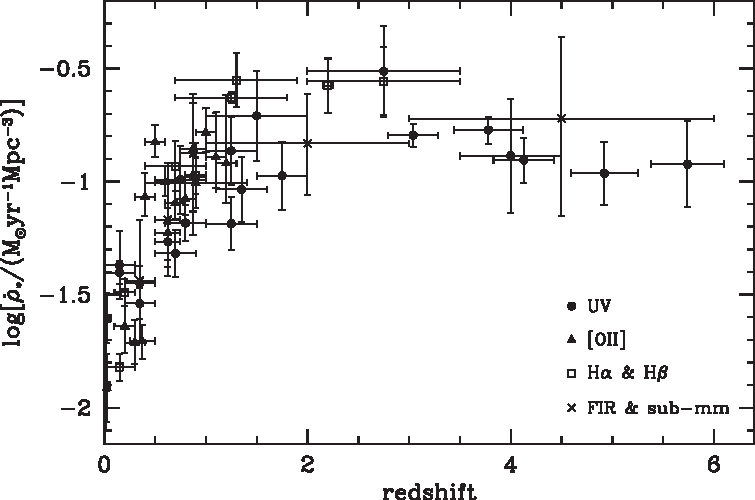
\includegraphics[width=0.7\textwidth]{img/ch-05/star-formation-rate.pdf}
	\caption{The global star formation rate as a function of redshift, from \cite{galaxy-formation}. We see that the star formation rate was mostly constant at redshifts earlier than $2$, but then dropped quickly until today.}
	\label{fig:star-formation-rate}
\end{figure}
We want to calculate the global rate of star formation $\dot{\rho}_\star(z)$, which is total gas mass turned into stars at redshift $z$ per unit time and volume. It can be estimated as
\begin{align*}
	\dot{\rho}_\star(z)
	&= \int   \avg{\dot{M}_\star}(L, z) \phi(L, z) \dd{L},
\end{align*}
where
\begin{itemize}
	\item $\avg{\dot{M}_\star}(L,z)$ is the star formation rate for galaxies with luminosity $L$ at redshift $z$, and
	\item $\phi(L, z)$ is the galaxy luminosity function, which is the number of galaxies formed per volume and luminosity.
\end{itemize}

\Cref{fig:star-formation-rate} shows that the global star formation rate has dropped since $z \approx 2$.

\section{Modelling galaxy formation}
In this section, we describe a basic framework for galaxy formation models, which should answer several questions:
\begin{itemize}[nolistsep]
	\item How can we model baryonic structure formation, and galaxy formation in particular?
	\item How can we account for the diversity and statistical properties of galaxies?
\end{itemize}
This is still an unsolved problem, and involves many interlinked processes.
To our cosmological model, which describes background expansion and the evolution of dark matter, we add the treatment of baryons.

\subsection{Gas cooling}
Gas can cool through different processes:
\begin{itemize}
	\item  Hot gas (hotter than \SI{107}{\kelvin}) in massive haloes is fully ionised and can cool through thermal bremsstrahlung (Cf. X-ray emission of galaxy clusters).
	At high redshift $(z 
	\geq 6)$, cooling can also proceed via inverse compton scattering of CMB photons by electrons
	\item Warm gas (\SIrange{e4}{e6}{\kelvin}) is partially ionised and can cool via atomic excitation and de-excitation mechanisms.
	The cooling rate depend strongly on chemical composition.
	\item Cold gas (colder than \SI{e4}{\kelvin}) is almost completely neutral, which suppresses the above cooling processes.
	Cooling is still possible by collisional (de-)excitation (heavy elements) or rotational/vibrational lines (molecules).
\end{itemize}

These cooling mechanisms (except inverse Compton scattering) involve two particles and are therefore more effective in higher density regions.

If cooling is effective (short cooling time), the gas accretes directly onto a central proto-galaxy.
If cooling time is long, the gas settles into hydrostatic equilibrium with halo (inner region can still cool and flow to the centre region)

If the DM halo has angular momentum, the gas can spin up as it flows inward yielding a cold disk at the centre of the halo -> disk galaxy


\subsection{Star formation}

As the gas flows to the centre of the DM halo, its self-gravity will eventually dominate the DM gravity.
This will lead to a runaway collapse of the gas which can then fragment and form stars.

Star formation is not well understood but can be characterised by the star formation rate $\dot{M}_{*}$ and the Initial Mass Function (IMF).
The stellar population can then be evolved using stellar evolution.
Star formation can be quiescent (in gas disks) or starburst (with accumulation of gas in small volumes, which can be triggered by interactions or instability.


\subsection{Feedback}
\begin{figure}
	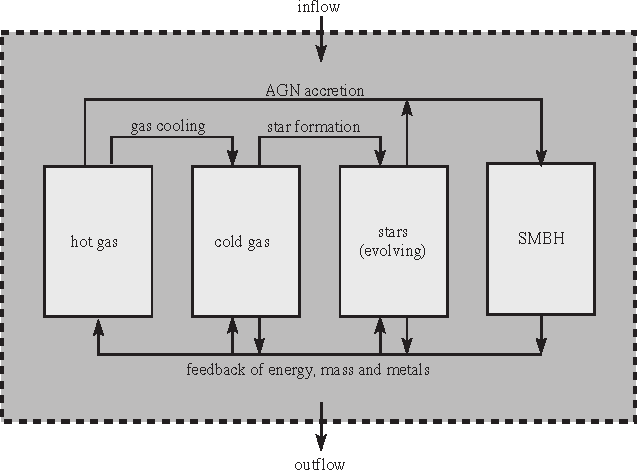
\includegraphics[width=0.8\textwidth]{img/ch-05/feedback.pdf}
	\caption{A flowchart of the evolution of an individual galaxy, from \cite{galaxy-formation}. The galaxy is represented by the dashed box which contains hot gas, cold gas, stars and a supermassive black hole (SMBH). Gas cooling converts hot gas into cold gas, star formation converts cold gas into stars, and dying stars inject energy, metals and gas into the gas components. In addition, the SMBH can accrete gas (both hot and cold) as well as stars, producing AGN activity which can release vast amounts of energy which affect primarily the gaseous components of the galaxy. Note that in general the box will not be closed: gas can be added to the system through accretion from the intergalactic medium and can escape the galaxy through outflows driven by feedback from the stars and/or the SMBH. Finally, a galaxy may merge or interact with another galaxy, causing a significant boost or suppression of all these processes.}
	\label{fig:feedback}
\end{figure}
Feedback processes inject energy, mass and metals into the gas.
Both supernova explosions at the end of stellar evolution and \ac{agn} can act as feedback processes.
They can reheat cold gas and thus suppress star formation, which is called negative feedback, or compress surrounding gas with shock waves and thus enhance star formation, which is called positive feedback.
\Cref{fig:feedback} shows the feedback processes that can occur in a galaxy.

\subsection{Mergers}

Baryons are also effected by mergers. Depending on the masses of the merging haloes, different effects occur.

If two halos of similar masses merge, violent relaxation quickly leads to a relaxed state for the new halo.
Hot gas from the progenitors is shock-heated and settles into hydrostatic equilibrium with the \ac{dm} halo potential.
Central galaxies, if present, merge to a new central galaxy, which is likely an elliptical galaxy.

If merging haloes have very different masses, the smaller halo orbits the main halo as a satellite until dynamical friction\sidenote{(Kinetic energy is transferred from a small object to a large object, making the small object sink towards the large one as it loses energy)} and tidal effects dissolve it.

In the limit of very small haloes merging into large halo, the accretion can be thought of as smooth accretion.


\subsection{Dynamical evolution}

As satellite galaxies orbit within dark matter halos, tidal interactions and pressure from the gas in the halo, called \emph{ram pressure}, can remove dark matter, gas and stars from the satellite.
These effects drive galaxy evolution in groups and clusters of galaxies and play a role in the environment dependence of galaxy properties.

Internal instabilities can also affect galaxy morphologies. 
In particular, a bar instabilities may develop in spiral galaxies, which can then buckle to create a pseudo-bulge. 
Bulges may therefore be remnants of either early stages of galaxy formation, or results from the buckling of a bar.

\subsection{Chemical evolution}

Heavy elements (metals) are produced in stars and expelled by supernovae explosions and stellar winds into the \ac{ism}. This has important implications for the evolution of the galaxy:

\begin{itemize}
	\item The cooling efficiency depends strongly on the metallicity, as cooling is more efficient for metal-enriched gas.
	\item Metallicity affects colour and luminosity of stellar population in galaxies.
	\item Small particles of heavy elements, called dust, can absorb starlight and reradiate it in the IR.
	This effect leads to \emph{extinction}, which makes all objects behind dust appear redder and dimmer than otherwise expected.
\end{itemize}


\subsection{Stellar population synthesis}
The spectrum of galaxies is mostly a combination of the spectra of many stars. Given the star formation rate $\dot{M}_{*}(z)$ and the \ac{imf}, the stellar population can be evolved using stellar evolution to derive a stellar synthesis spectrum. The effect of gas emission and absorption, dust extinction, and \ac{agn} emission also need to be modelled.


\subsection{Intergalactic Medium}

The \ac{igm} also plays an important role in galaxy formation through the inflow and outflow of baryons.




\subsection{Time Scales}
\begin{itemize}
	\item Hubble time: current expansion rate time scale ($H^{-1}$)
	\item Dynamical time: time to orbit across steady state dynamical system
	\item Cooling time: ratio between thermal energy to energy loss rate of gas
	\item Star formation time: ratio of cold gas content and star formation rate
	\item Chemical enrichment time: time scale on which gas is enriched in heavy elements
	\item Merging time: typical time before major merger
	\item Dynamical friction time: time scale for a satellite in large halo to lose its orbital energy and merge to centre
\end{itemize}


\subsection{Examples}
\begin{itemize}
	\item Processes whose time scale is larger than the Hubble time can be ignored (For example dynamical friction time for satellite galaxies with masses much smaller than the parent halo $>$ Hubble time $\rightarrow$ Clusters of galaxies have numerous member galaxies)
	\item If cooling time > dynamical time, the hot gas will typically be in Hydrostatic equilibrium. In the opposite case, the gas will cool rapidly and sink to the halo centre without establishing hydrostatic equilibrium
	\item If star formation time is comparable to dynamical time, gas will turn into stars during the the collapse, likely leading to an elliptical galaxy. If star formation time is larger than cooling and dynamical time then, the gas will settle into rotationally supported disk before forming stars likely leading to a disk galaxy (angular momentum also plays a role)
	\item If chemical evolution time is larger than the star formation time, little enrichment will occur during star formation and stars will end up with the same initial metallicity. In the opposite case, the gas is continually enriched and stars will have different metallicities depending on formation time.
\end{itemize}

A flow chart to determine the evolution of a galaxy is shown in \cref{fig:galaxy-decision}.

\begin{figure}
	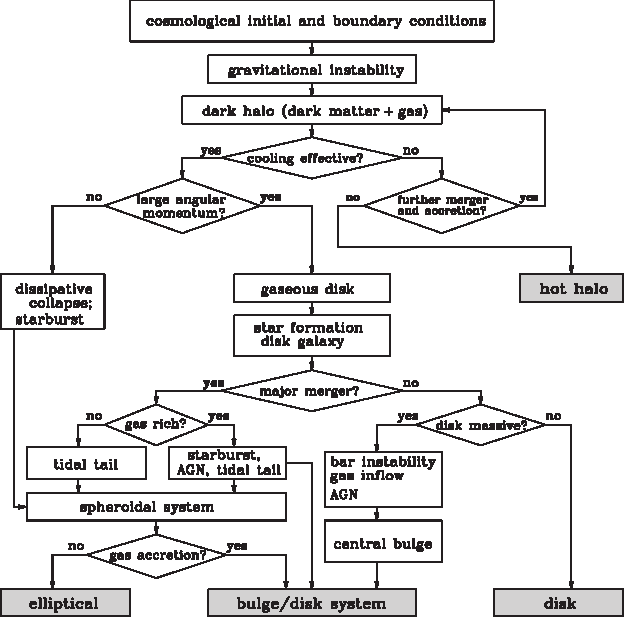
\includegraphics[width=0.8\textwidth]{img/ch-05/galaxy-decision.pdf}
	\caption{A logic flow chart for galaxy formation, from \cite{galaxy-formation}. In the standard scenario, the initial and boundary conditions for galaxy formation are set by the cosmological framework. The paths leading to the formation of various galaxies are shown along with the relevant physical processes. Note, however, that processes do not separate as neatly as this figure suggests. For example, cold gas may not have the time to settle into a gaseous disk before a major merger takes place.}
	\label{fig:galaxy-decision}
\end{figure}


\section{Modelling schemes}

\subsection{Semi-analytical models}
\begin{itemize}
	\item Use N-body simulations (DM only) or Extended Press-Schechter to generate halo merger tree
	\item For each halo track the hot gas, cold gas and stars
	\item Use prescriptions to convert these components into one another and their metallicity (model cooling, star formation, feedback and chemical evolution
	\item Use prescription for the evolution of these components in mergers and for the survival of satellites in parent halos.
\end{itemize}
Relatively fast procedure with can then be compared to observations.

\subsection{Hydrodynamical simulations}
\begin{itemize}
	\item Use N-body+hydrodynamical simulations to model the DM, the gas and stars.
	\item As simulations are limited by resolution, prescription are needed for sub-grid physics, such as cooling, star formation and evolution, feedback, chemical evolution
\end{itemize}
More computationally intensive but avoids semi-analytical halo modelling.
Can then also be compared to observations.
